\documentclass[preview]{standalone}

\usepackage{amsmath,amsfonts,amsthm}
\usepackage[english]{babel} 
\usepackage[hscale=0.7,vscale=0.8]{geometry}
\usepackage[square,numbers]{natbib}

\usepackage{graphicx}
\usepackage{subcaption}
\usepackage{tikz}

\usetikzlibrary{shapes.misc, positioning}
\usetikzlibrary{fit,positioning}
\usetikzlibrary{bayesnet}

\begin{document}


\begin{align*}	
\mathbf{z} \sim \qquad  \qquad
\begin{tikzpicture}[transform canvas={scale=.65}]
	\node[latent, ultra thick] (z1) {};	
	\node[latent, ultra thick, above right = .25cm and 1cm of z1] (z2) {};	
	\node[latent, ultra thick, above left = .25cm and 1cm of z1] (z3) {};;
	\draw [thick] (z1) -- (z2);
	\draw [thick] (z1) -- (z3);
\end{tikzpicture} \\
\boldsymbol \gamma \mid \mathbf{z} & \sim  \qquad\mathcal{N}(\boldsymbol \mu_{\mathbf{z}}, \sigma^2 \mathbf{I}) \\
\mathbf{y} \mid \boldsymbol \gamma & \sim  \qquad\mathbb{P}\left( h\left( \boldsymbol \gamma \right) \right)
\end{align*}	

\end{document}





